\documentclass[journal,twoside,web]{ieeecolor}
\usepackage{generic}
\usepackage{cite}
\usepackage{amsmath,amssymb,amsfonts}
\usepackage{algorithmic}
\usepackage{graphicx}
\usepackage{algorithm,algorithmic}
\usepackage{hyperref}
\hypersetup{hidelinks=True}
\usepackage{textcomp}
\usepackage{subcaption}
%Added by Cheng
% \usepackage{multirow,array,enumitem,adjustbox}
\usepackage{booktabs,threeparttable,makecell}

\def\BibTeX{{\rm B\kern-.05em{\sc i\kern-.025em b}\kern-.08em
    T\kern-.1667em\lower.7ex\hbox{E}\kern-.125emX}}
\markboth{\hskip25pc IEEE TRANSACTIONS AND JOURNALS TEMPLATE}
{Author \MakeLowercase{\textit{et al.}}: Title}
\begin{document}
\title{Enhancing Alzheimer's Disease Diagnosis and Progression Prediction Through Multimodal Integration}
% \author{}
% \thanks{ is with the Department of (e-mail: ). }


\maketitle

\begin{abstract}
Alzheimer’s Disease (AD) classification methodologies increasingly use machine learning and deep learning. There is a gap in literature in using Vision Transformers (ViT) and hybrid vision transformer-convolutional neural net-vision transformers (ViT-CNN) in the multimodal prediction of AD using brain imaging. This study aims to: 1) classify AD status into 3 classes, 2) predict AD progression across 7 time-points, and 3) assess multimodal data integration's impact. Our approach combines CNNs and ViT for feature extraction from MRI, PET, EHR, and Genetic data, followed by feature fusion and classification. The hybrid ViT-CNN achieves 77\% validation and 70\% testing accuracy, outperforming individual models for AD classification. On the other hand, CNN (48-62 \%) outperforms the ViT (43-59 \%)  and the hybrid model (44-60 \%) for AD progression across seven timepoints on testing accuracy.  
Results indicate that PCA offers no benefit for AD progression classification, and SVM with 50 components performs best. Modality combination increases accuracy but decreases test sensitivity. Conclusion: The hybrid ViT-CNN model shows promise for AD classification not AD progression, extracting rich features from multimodal data. However, modality combination impacts sensitivity differently for CNN and ViT models.
\end{abstract}

\begin{IEEEkeywords}
Convolutional Neural Network, Vision Transformers, ADNI, Alzheimer's Disease, Support Vector Machine, Principal Component Analysis\
\end{IEEEkeywords}

\section{Introduction: Multimodal Approaches to Alzheimer’s Disease Prediction.}
\label{sec:introduction}
\IEEEPARstart{T}{here} are 55 million people worldwide living with dementia, with 10 million new cases every year \cite{who_dementia_nodate}. Alzheimer's Disease (AD) is the most common type of dementia, accounting for 60-70\% of cases \cite{who_dementia_nodate}. With the growing number of cases, there is a growing interest in using AI models to classify AD cases and predict the progression of AD longitudinally with varying levels of success. Different types of AI have been analyzed in various ways to determine if there is a superior methodology for multimodal AD classification.

% AI models have shown promise in the early detection of AD, particularly in distinguishing between Mild Cognitive Impairment (MCI) and Normal Control (NC), as well as between MCI and AD. Machine learning and deep learning approaches, such as support vector machines (SVM) and convolutional neural networks (CNN), have been employed with notable success. Combining multiple modalities, such as Magnetic Resonance Imaging (MRI) and Positron Emission Tomography (PET), has been shown to enhance classification accuracy compared to using a single modality.

\subsection{Multimodal Alzheimer's Disease Classification}
There is a growing interest in using machine learning and deep learning approaches for early detection of Alzheimer's Disease (AD, \cite{lin_convolutional_2018}, \cite{grueso_machine_2021}, \cite{borchert_artificial_2021}). The Mild Cognitive Impairment (MCI) is when adults have more memory or thinking problems than adults their age, while the symptoms are not as sever as dementia and AD \cite{NationalInstituteOfAging_MildCognitiveImpairment_2024}.   A review paper by Grueso and Viejo-Sobera found the best performing machine learning method to classify MCI vs. Normal to be a support vector machine (SVM), with a mean accuracy of 75.4\%, and the best performing deep learning model to be a convolutional neural network (CNN), with a mean accuracy of 78.5\% \cite{grueso_machine_2021}. They found that most studies combined MRI and PET images to increase their classification accuracies compared to just using one modality \cite{grueso_machine_2021}\cite{borchert_artificial_2021}. 

Researchers have proposed different ways of integrating information and features from MRI and PET. Initially, Hinrichs and colleagues worked on multi-kernel learning \cite{hinrichs_predictive_2011}, Zhang and Shen on kernel combinations \cite{zhang_multi-modal_2012}, and Young and colleagues on the Gaussian Process with mixed kernel \cite{young_accurate_2013}. More recently, Lu and colleagues have developed custom deep neural networks \cite{lu_multimodal_2018}, Zhu and colleagues on low-rank dimensionality reduction and orthogonal rotation in a sparse linear regression framework \cite{zhu_low-rank_2019}, Gupta and colleagues on kernel-based approaches \cite{gupta_prediction_2019}, Zhou and colleagues on latent representational learning \cite{zhou_latent_2019}, Shao and colleagues on a hypergraph-based multi-task feature selection \cite{shao_hypergraph_2020},\cite{zu_label-aligned_2016} Zu and colleagues on a novel sparse regression to fuse imaging data with auxiliary data \cite{shen_heterogeneous_2021}, Song and colleagues on image fusion \cite{song_effective_2021}, and Singh and colleagues on feature and intermediate-level fusion methods \cite{singh_multi-modal_2023}.

Song et al. \cite{song_effective_2021} proposed a novel image fusion approach to integrate information from MRI and PET scans for improved AD diagnosis. They performed skull-stripping on structural MRI scans to remove non-brain tissue and reduce noise, registered the MRI to a standard brain atlas template, segmented GM tissue from the registered MRI, co-registered the FDG-PET image to the corresponding registered MRI, and extracted the corresponding GM area from the co-registered PET image. This combined information from two images improved AD diagnosis.

\subsection{Multimodal Alzheimer's Disease Progression}
In addition to classification, tracking the progression of AD over time is crucial for understanding disease development and improving patient management. Cheng et al. \cite{cheng_multimodal_2015} used sparse multimodal manifold-regularized transfer learning for MCI conversion prediction. Their method includes a criterion based on maximum mean discrepancy for eliminating the negative effect of the difference between AD/NC and pMCI/sMCI, and a sparse semi-supervised manifold-regularized least squares classification method. Other researchers have used autoregressive modeling of multimodal biomarkers \cite{minhas_predicting_2018}, and an Extreme Learning Machine (ELM)-based grading method where features extracted from MRI were combined with ELM gradings of MRI, PET, CSF, and genetic data and then fed into a classifier \cite{lin_predicting_2020}.

Researchers have proposed various methods for integrating multimodal data, including multi-kernel learning, custom deep neural networks, low-rank dimensionality reduction, and feature fusion techniques. Further exploring multimodality in Alzheimer's disease research, V. Adarsh et al. introduced a custom kernel to classify different stages of Alzheimer’s disease and MCI using a multimodal approach by combining imaging data with patient clinical data \cite{adarsh_multimodal_2024}. The model was evaluated on the Alzheimer’s Disease Neuroimaging Initiative (ADNI) dataset using multiple metrics, including AUC, ROC, accuracy, sensitivity, recall, and precision. The integration of LIME and CAM software improved the transparency of the model, enhancing precision, accuracy, and recall.

C. Ellis Wisley et al. \cite{wisely_convolutional_2022}utilized CNN to extract features from retinal images, combining different types of retinal images in a CNN for feature extraction. The model was evaluated on an AUC curve, achieving an AUC of 0.861 on the validation set and 0.841 on the test set, demonstrating potential clinical applications for Alzheimer's disease diagnosis. 

There is a gap in the literature in using Vision Transformers (ViT) and hybrid CNN-ViT models. ViT uses less computational resources than CNN, it is better at understanding global image context, learns from image sequences and outperforms CNN on large datasets \cite{dosovitskiy_image_2021}. On the other hand, CNN are good at extracting local features. Combinig these two models theoretically can extract both local and global image contexts and Improve AD classification and progression performance. 

\subsection{Evaluation of Multimodal Contributions to AD Classification and Progression Prediction}
The first goal of this proposal is to investigate the use of multimodal integration methods (i.e., feature-level fusion) for the classification of AD vs. MCI and MCI vs. NC. By harnessing the power of AI models and leveraging multimodal datasets, we aim to enhance diagnostic accuracy, prognostic capability, and ultimately, patient care outcomes. The third aim of this project is to assess how combining MRI, PET, Electronic Health Records (EHR), and genetic data (e.g., Polygenic Hazard Score, PHS \cite{desikan_genetic_2017}) improves classification performance.

Based on the literature, it is unclear whether MRI or PET contributes more to classification performance. In two separate studies, one by Wisely and colleagues comparing PET to MRI \cite{wisely_convolutional_2022} and one by Zhang and colleagues comparing PET/CT to MRI \cite{zhang_petmr_2017}, it was found that separating these modalities provided equal insights into AD classification and progression. However, combining PET and MRI provided new insights as the structural and functional components of the scans were combined, offering enhanced information. 

By integrating advanced AI techniques with multimodal data, this research aims to provide a comprehensive approach to AD diagnosis and progression tracking. The ultimate goal is to improve patient outcomes by enabling earlier and more accurate detection of AD and its progression. The contributions of this paper are as follows:
\begin{itemize}
    \item \textbf{Multimodal Integration for AD Classification:}
    We developed a hybrid approach combining Convolutional Neural Networks (CNN) and Vision Transformers (ViT) for feature extraction from MRI, PET, EHR, and Genetic data. In addition, we implemented feature-level fusion techniques to classify Alzheimer's Disease (AD) status into three classes: Normal Control (NC), Mild Cognitive Impairment (MCI), and AD.
    
    \item \textbf{Prediction of AD Progression:}
    We evaluated CNN, ViT, CNN-ViT's ability to predict AD progression across seven time-points. Furthermore, we analyzed the performance of multimodal data integration on the accuracy and sensitivity of AD progression prediction.
    
    \item \textbf{Impact of Modality Combination:}
    We investigated the effects of combining different modalities on model performance, finding that while modality combination increases overall accuracy, it decreases test sensitivity. In addition, we provided insights into how different modalities and their combinations affect the sensitivity of CNN and ViT models differently.

 
\end{itemize}\ 

 
%\vspace{-2mm}

% \section{Related Work}
\label{sec:related}
\subsection{Alzheimer's Disease Classification}
There is a growing interest in using machine learning and deep learning approaches for early detection of Alzheimer's Disease (AD, \cite{lin_convolutional_2018}, \cite{grueso_machine_2021}, \cite{borchert_artificial_2021}). The early stage of AD is called Mild Cognitive Impairment (MCI). A review paper by Grueso and Viejo-Sobera found the best performing machine learning method to classify MCI vs. Normal to be a support vector machine (SVM), with a mean accuracy of 75.4\%, and the best performing deep learning model to be a convolutional neural network (CNN), with a mean accuracy of 78.5\% \cite{grueso_machine_2021}. They found that most studies combined MRI and PET images to increase their classification accuracies compared to just using one modality \cite{grueso_machine_2021}\cite{borchert_artificial_2021}.

Researchers have proposed different ways of integrating information and features from MRI and PET. Initially, researchers worked on multi-kernel learning \cite{hinrichs_predictive_2011}, kernel combinations \cite{zhang_multi-modal_2012}, and the Gaussian Process with mixed kernel \cite{young_accurate_2013}. More recently, researchers have developed custom deep neural networks \cite{lu_multimodal_2018}, low-rank dimensionality reduction and orthogonal rotation in a sparse linear regression framework \cite{zhu_low-rank_2019}, kernel-based approaches \cite{gupta_prediction_2019}, latent representational learning \cite{zhou_latent_2019}, a hypergraph-based multi-task feature selection \cite{shao_hypergraph_2020},\cite{zu_label-aligned_2016} a novel sparse regression to fuse imaging data with auxiliary data \cite{shen_heterogeneous_2021}, image fusion \cite{song_effective_2021}, and feature and intermediate-level fusion methods \cite{singh_multi-modal_2023}.

Song et al. \cite{song_effective_2021} proposed a novel image fusion approach to integrate information from MRI and PET scans for improved AD diagnosis. They performed skull-stripping on structural MRI scans to remove non-brain tissue and reduce noise, registered the MRI to a standard brain atlas template, segmented GM tissue from the registered MRI, co-registered the FDG-PET image to the corresponding registered MRI, and extracted the corresponding GM area from the co-registered PET image. This combined information from two images improved AD diagnosis.

\subsection{Alzheimer's Disease Progression}
Cheng et al. \cite{cheng_multimodal_2015} used sparse multimodal manifold-regularized transfer learning for MCI conversion prediction. Their method includes a criterion based on maximum mean discrepancy for eliminating the negative effect of the difference between AD/NC and pMCI/sMCI, and a sparse semi-supervised manifold-regularized least squares classification method. Other researchers have used autoregressive modeling of multimodal biomarkers \cite{minhas_predicting_2018}, and an Extreme Learning Machine (ELM)-based grading method where features extracted from MRI were combined with ELM gradings of MRI, PET, CSF, and genetic data and then fed into a classifier \cite{lin_predicting_2020}.

Further exploring multimodality in Alzheimer's disease research, V. Adarsh et al. introduced a custom kernel to classify different stages of Alzheimer’s disease and MCI using a multimodal approach by combining imaging data with patient clinical data \cite{adarsh_multimodal_2024}. The model was evaluated on the Alzheimer’s Disease Neuroimaging Initiative (ADNI) dataset using multiple metrics, including AUC, ROC, accuracy, sensitivity, recall, and precision. The integration of LIME and CAM software improved the transparency of the model, enhancing precision, accuracy, and recall.

C. Ellis Wisley et al. \cite{wisely_convolutional_2022}utilized CNN to extract features from retinal images, combining different types of retinal images in a CNN for feature extraction. The model was evaluated on an AUC curve, achieving an AUC of 0.861 on the validation set and 0.841 on the test set, demonstrating potential clinical applications for Alzheimer's disease diagnosis.

\subsection{Modality Contribution}
Based on the literature, it is unclear whether MRI or PET contributes more to classification performance. In two separate studies, one comparing PET to MRI \cite{wisely_convolutional_2022} and one comparing PET/CT to MRI \cite{zhang_petmr_2017}, it was found that separating these modalities provided equal insights into AD classification and progression. However, combining PET and MRI provided new insights as the structural and functional components of the scans were combined, offering enhanced information. 
% \vspace{-3mm}

\section{Methodology}
\label{sec:method}
\subsection{ADNI Dataset}
The datasets used in the preparation of this article were obtained from the Alzheimer’s Disease Neuroimaging Initiative (ADNI) database \cite{lu_multimodal_2018}. The ADNI was launched in 2003 as a public-private partnership, led by Principal Investigator Michael W. Weiner, MD. The primary goal of ADNI has been to test whether serial magnetic resonance imaging (MRI), positron emission tomography (PET), other biological markers, and clinical and neuropsychological assessment can be combined to measure the progression of mild cognitive impairment (MCI) and early Alzheimer’s disease (AD). De-identified patient data was obtained and were placed into a server where the images could be accessed for pre-processing and use in the pipeline. The dataset used for AD Classification was obtained by the search criteria ADNI phase 1, Subjects: MCI, AD and CN, subjects with both PET and MRI (Axial) and chosen original images. In total there are 1006 images (450 MCI, 244 CN, and 312 AD) for 233 patients. In addition, we found that the MRI images from this dataset were masks and used a previously downloaded MRI with PET images from this dataset.   This hybrid dataset has 2102 images (1166 MCI, 515 CN, and 421 AD) for 290 patients.  

The dataset used for AD Progression was obtained by searching criteria ADNI, Subjects: MCI, AD and CN, modalities: subjects with PET or MRI. Then we filtered for subjects with both MRI and PET images such that the images have been through their preprocessing steps. For PET the preprocessing steps are co-registration, averaging, standardization of voxel sizes and uniforming the resolution.  The MRI preprocessing steps are intensity normalization and scaling. This dataset has 3177 images. Then the subjects’ images were divided into 7 timepoints based on their visit label and if from one timepoint to the next their diagnosis label didn’t change, a new label of stable MCI (sMCI) were created for them, otherwise if their diagnosis had changed, they got the new label of progressive MCI (pMCI). There are 521 sMCI and 466 pMCI

\subsection{AD Classification}
\begin{figure}
    \centering
    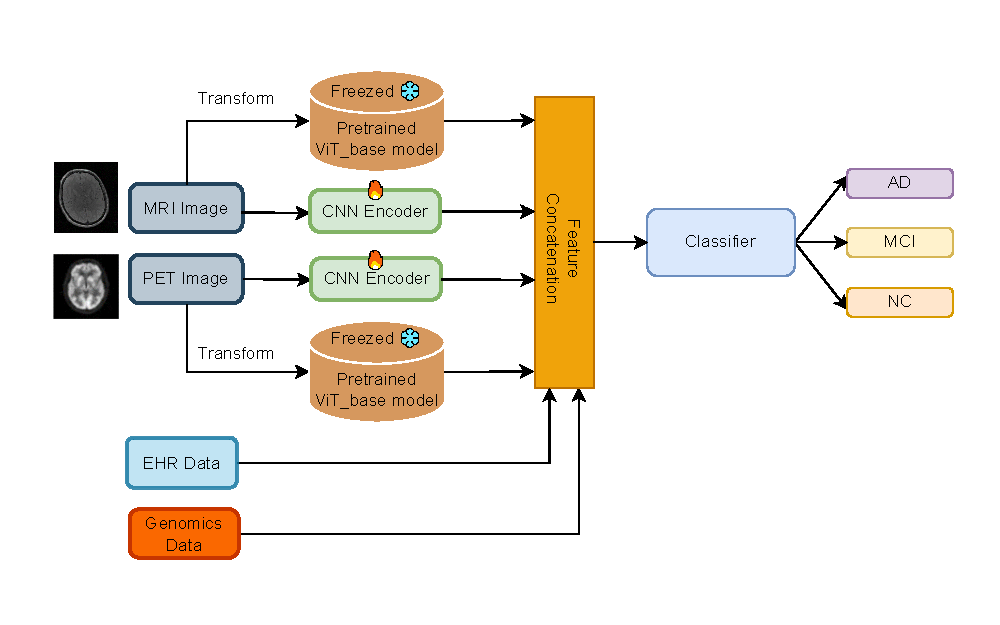
\includegraphics[width=1\linewidth]{figs/arch-classification_new.pdf}
    % \vspace{-2mm}
    
    \caption{Proposed architecture for multimodal AD classification}
    \vspace{-2mm}
    \label{fig:enter-label}
\end{figure}
In this study, we propose a novel classification method for AD that utilizes CNN and vision transformer (ViT\cite{dosovitskiy_image_2021}) to extract features of each modality and combine them for AD classification. The method combines two imaging modalities: MRI and PET. The architecture of our model is shown in Figure 1. For each modality (MRI and PET), the feature extraction with CNN is a custom architecture consisting of two convolution layers with ReLU and pooling. Then, we use the pre-trained ViT model to capture global and long-range dependencies. The preprocessing includes reshaping the 3D image data and select the first channel to adapt to the ViT input format, and then extract the features. 

Next, we did feature fusion using concatenation and multiplicative methods. The concatenation method combines the MRI and PET features from CNN and ViT together to form a combined feature representation. This combined feature then passes through two fully connected layers, and finally outputs the AD classification result (AD, MCI or NC). During the training process, the entire model is optimized in an end-to-end manner. 

The AD Progression pipeline consists of dividing the subjects’ visits into 7 timepoint pairs (t to t+1). The feature extraction for MRI and PET were done using either a pretrained convolutional neural net (CNN, ResNet18) or a pretrained Vision Transformer (ViT, vit-base-patch16-224). The feature extraction for EHR sex was done by converting it to 0 (female) or 1 (male), and for age it was normalized to values from 0 to 1. The Genetic data used is the Polygenic Hazard Score (PHS) which is a score based on APOE and 31 other genetic variants \cite{desikan_genetic_2017}. The PHS was normalized from 0 to 1. The next step is Feature Fusion where the PHS and along with EHR (sex and age), PET (1000 features) and MRI (1000 features) were combined in a feature matrix such that each subject had 2003 features. Then we did dimensionality reduction using Principal Component Analysis (PCA) and then we did the classification using Support Vector Machine with linear kernel.  

The dataset for each timepoint was then split into training and testing using a 5-fold cross-validation (80:20 train-test split). The hyperparameter optimization was done on different number of components for PCA: 2, 10, 25 and different number of components for the SVM classifier: 1, 10, 50. 

The hybrid model architecture for the AD progression , named BrainModel, integrates a pre-trained ResNet18 convolutional neural network (CNN) and a Vision Transformer (ViT) to leverage the strengths of both architectures for image classification tasks. The ResNet18 model is utilized for its robust feature extraction capabilities from convolutional operations, with its final fully connected layer removed and replaced by an identity layer to extract features. The ResNet18 layers are partially frozen, allowing only the parameters in the last convolutional block (layer4) to be trainable, ensuring the early layers' learned representations remain intact while allowing adaptation of higher-level features.

Parallel to the ResNet18, the ViT model is employed to capture global context and spatial relationships in the image. The ViT is also pre-trained, with the early layers frozen and only the last two blocks' parameters set as trainable, enabling fine-tuning of the model to the specific task at hand. Features from both models are extracted and concatenated, forming a combined feature vector comprising 512 features from ResNet18 and 768 features from ViT.

This combined feature vector is then passed through a fully connected layer reducing the dimensionality to 256 features, followed by a dropout layer with a 50\% dropout rate to mitigate overfitting. The final layer is a fully connected layer that maps the 256 features to the target number of classes, which is 2 in this case. The overall architecture allows the model to harness the detailed local feature extraction of the CNN and the global context understanding of the ViT, resulting in a powerful hybrid model for image classification.

To enhance the performance and robustness of our hybrid model, we employed a two-stage transfer learning process using separate models for MRI and PET images. For the MRI images, we utilized the BrainModel architecture and performed transfer learning using the entire MRI dataset. This process involved fine-tuning the pre-trained ResNet18 and ViT models within the BrainModel, adjusting their trainable layers to the specific characteristics of MRI data. The refined MRI model, thus adapted, was subsequently used to extract high-level features from the MRI dataset, capturing both local and global patterns effectively.

Similarly, a separate BrainModel was employed for the PET images. This PET-specific BrainModel underwent transfer learning using the entire PET dataset, fine-tuning the pre-trained ResNet18 and ViT models to capture the unique attributes of PET data. The adapted PET model was then used to extract robust features from the PET images. These features, derived from separate MRI and PET models, were then combined in the hybrid model to leverage the complementary information from both imaging modalities.

The training process utilized a 10-fold cross-validation scheme to ensure robustness and generalization. This was achieved using the KFold class from scikit-learn, configured with 10 splits, shuffled data, and a fixed random state for reproducibility. The key hyperparameters for training included a learning rate of 0.001, a batch size of 4, and a total of 25 epochs. Additionally, a weight decay of 1e-4 was applied to regularize the model and prevent overfitting. This systematic approach ensured that the hybrid model was finely tuned and capable of effectively integrating the distinct features from MRI and PET images.

\subsection{Modality Contributions}
\textbf{AD Classification}
In this study, we explore the impact of various modalities on AD classification by employing different single and combined modalities. We utilized PET, MRI, EHR, and genomic data. Our methodology involves setting up distinct experimental conditions for each modality and combinations thereof, particularly focusing on MRI and PET due to their prevalent use in medical imaging. The multimodal model, combining MRI and PET, is further examined under various hyperparameter settings to gauge stability and effectiveness in AD classification. 

For in-depth learning the importance of different modality, we conduct feature permutation experiments in the multimodal ViT-CNN model to assess the individual contributions of each modality, we record the features of each different modality from different networks from the feature splicing layer (named mri-cnn, pet-cnn, mri-vit, pet-vit, ehr). To assess the importance of features from different modalities in AD classification, we employ the permutation importance method. First, we evaluate the trained model on the test set to obtain baseline accuracy. Then, for each feature in the CNN and ViT components of both MRI and PET modalities, we perform multiple iterations of feature permutation. In each iteration, we randomly shuffle the values of a single feature while keeping other features unchanged, and re-evaluate the model's accuracy on the test set. The difference between the permuted accuracy and the baseline accuracy is calculated as the importance score for that feature. Finally, we average the importance scores across all iterations to obtain the final importance measure for each feature. 

\textbf{AD Progression}
One important question in Multimodal AD classification and prediction is how much each modality is contributing to the classifications. This was tested for the AD Progression by just doing the classification based on features extracted from CNN vs. ViT from MRI, PET, MRI \& PET, EHR \& Genetic, and MRI \& PET \& EHR \& Genetic.
\begin{figure}
    \centering
    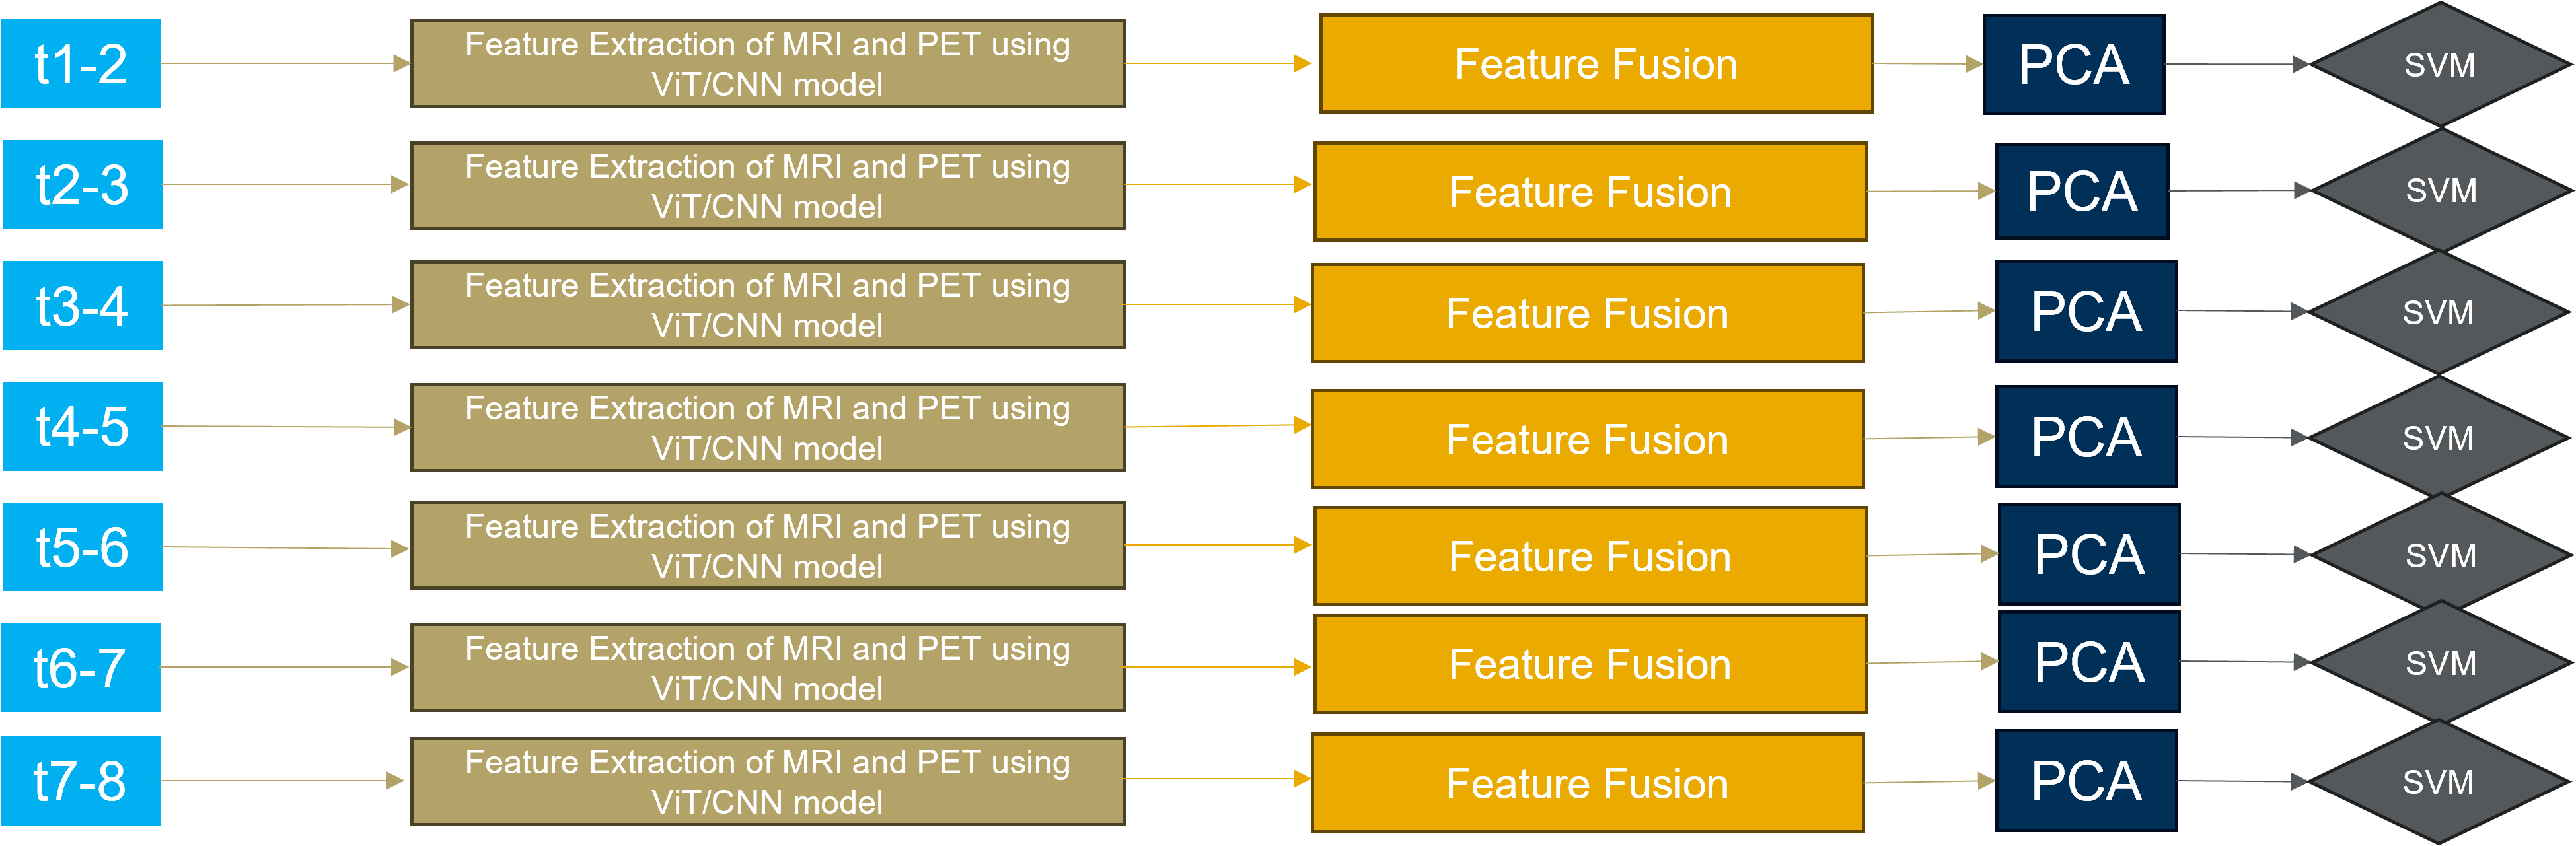
\includegraphics[width=1\linewidth]{figs/Picture14.png}
    \caption{Proposed architecture for multimodal AD Progression }
    \label{fig:enter-label}
\end{figure}
%\vspace{-2mm}

\section{Results}
\label{sec:results}
\subsection{AD Classification}
In this section, we use 5-fold cross-validation to evaluate the performance of the proposed model. Specifically, we randomly divided the data set into 5 subsets, selected 4 subsets as the training set each time, and the remaining 1 subset as the validation set. This process is repeated 5 times to ensure that each subset has a chance to serve as a validation set. We use the Adam optimizer, set the learning rate to 0.0001, and set the number of training epochs to 5. We adopt the cross-entropy loss function as the optimization objective. It is worth noting that our model is trained in multi-modal data, taking full advantage of the complementary information of MRI and PET images. 
%\begin{figure}
%    \centering
%    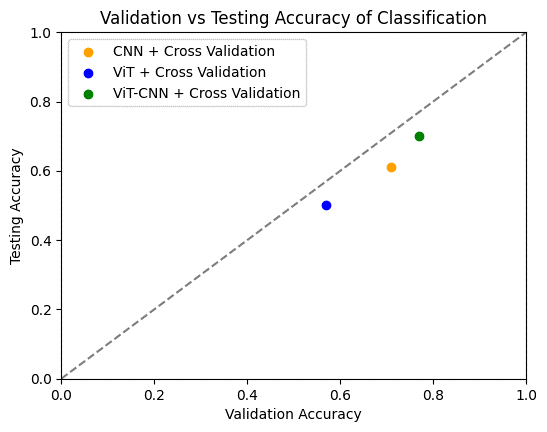
\includegraphics[width=1\linewidth]{figs/Picture13.png}
%    \caption{Predictivity plot for three different class (CN, MCI, and AD) in three models with 5cross-validation }
%    \label{fig:enter-label}
%\end{figure}

We compare the performance of three models for ablation study: CNN encoder model, ViT model and our proposed hybrid ViT-CNN model. Experimental results show that the hybrid ViT-CNN model achieved an accuracy of 77\% on the validation set, which is significantly better than the other two models. This proves that combining the advantages of CNN and ViT can effectively improve the performance of AD classification. In addition, we found that the hybrid ViT-CNN model showed better consistency, and its validation results were closer to the test results (validation accuracy 77\%, test accuracy 70\%). 

Comparison results for CNN-based model and hybrid ViT-CNN model revealed significant improvements in the hybrid ViT-CNN model's performance compared to the CNN-based approach. By incorporating a pretrained ViT alongside the CNN encoder, the hybrid model achieves a remarkable increase in sensitivity from approximately 52\% to around 80\%, while maintaining consistent hyperparameters. 
% \begin{figure}
%     \centering
%     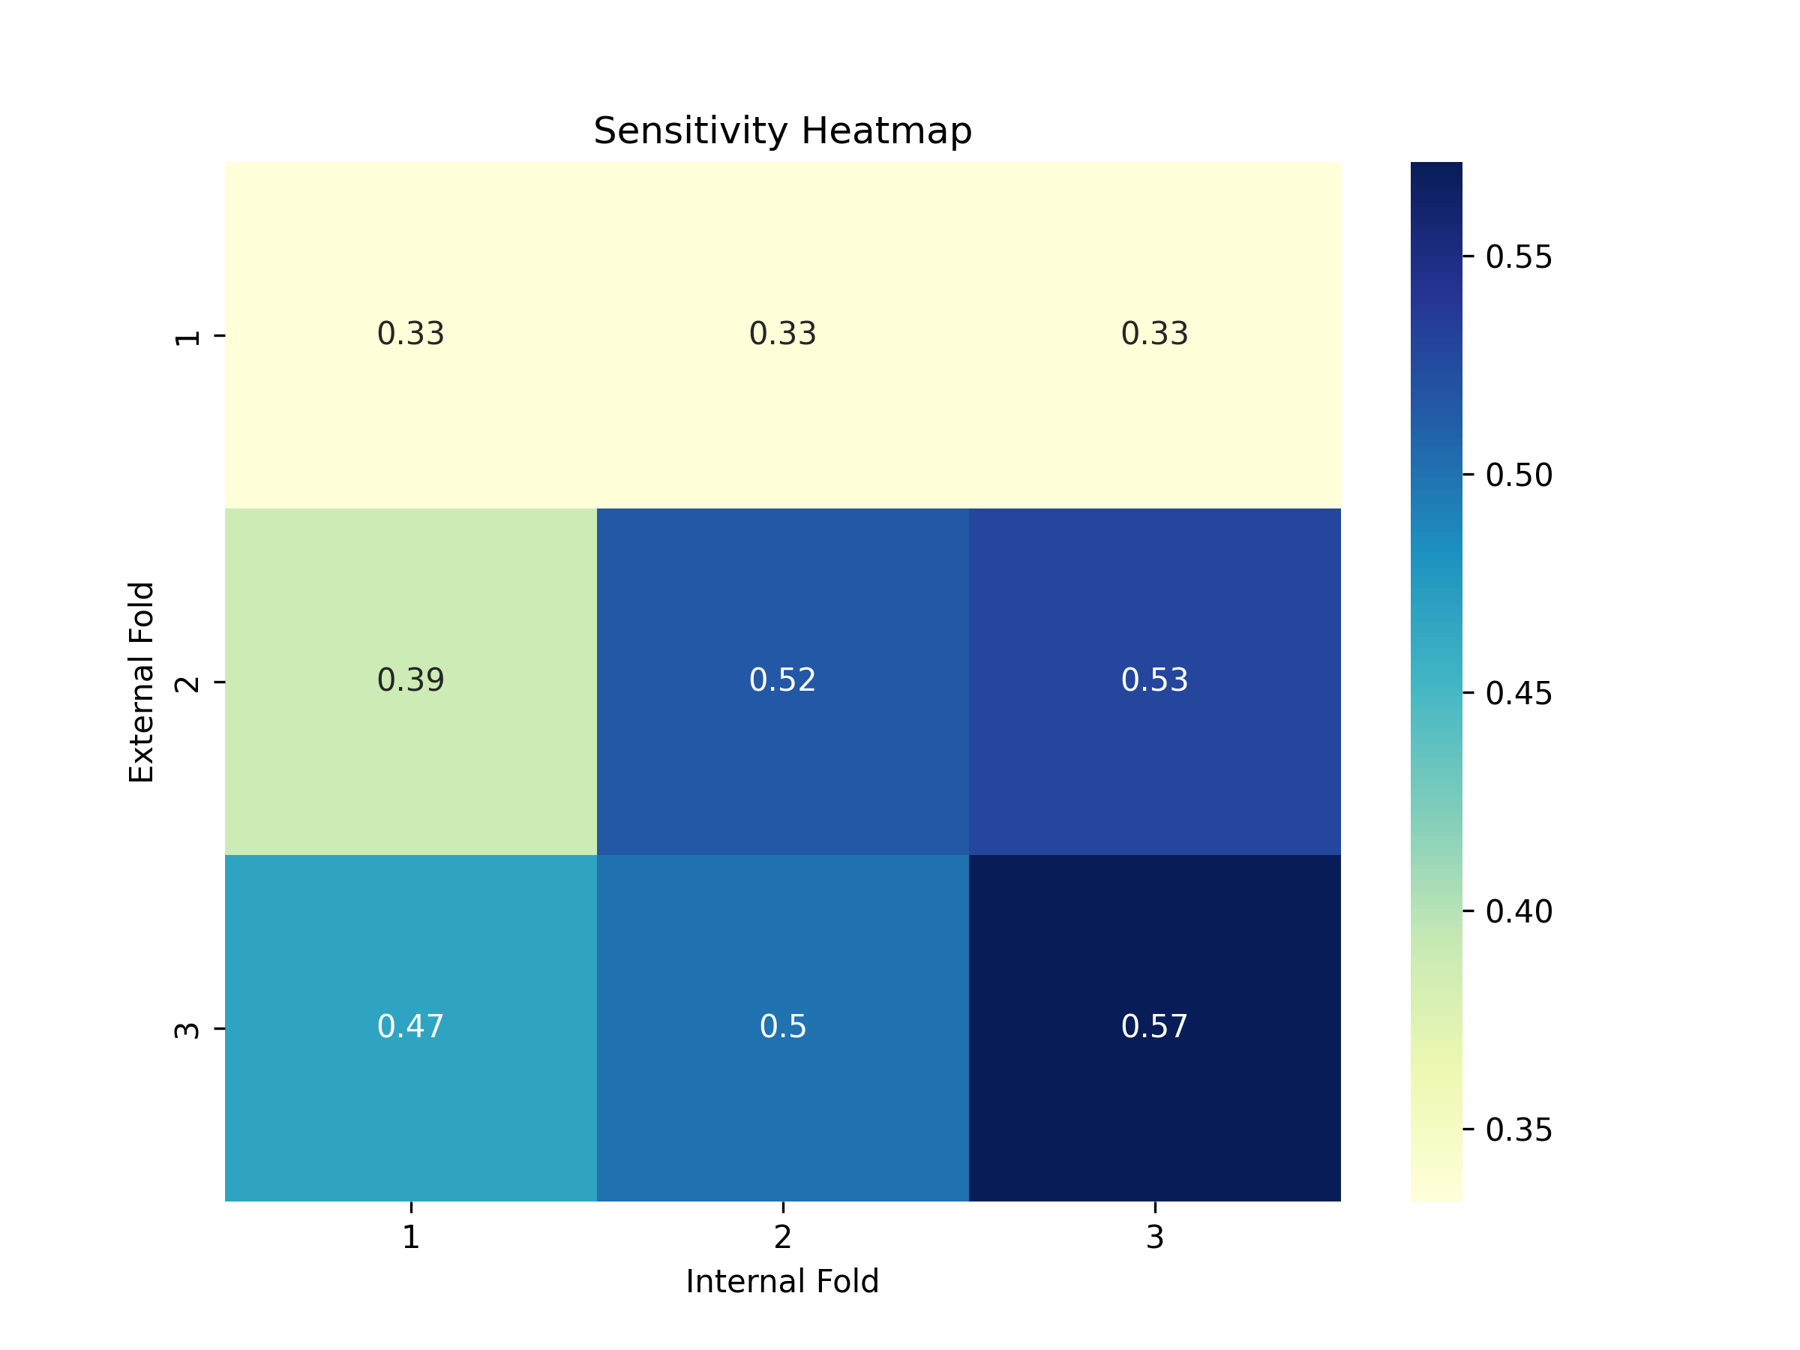
\includegraphics[width=1\linewidth]{figs/Picture3.png}
    
    
% \end{figure}
% \begin{figure}
%     \centering
%     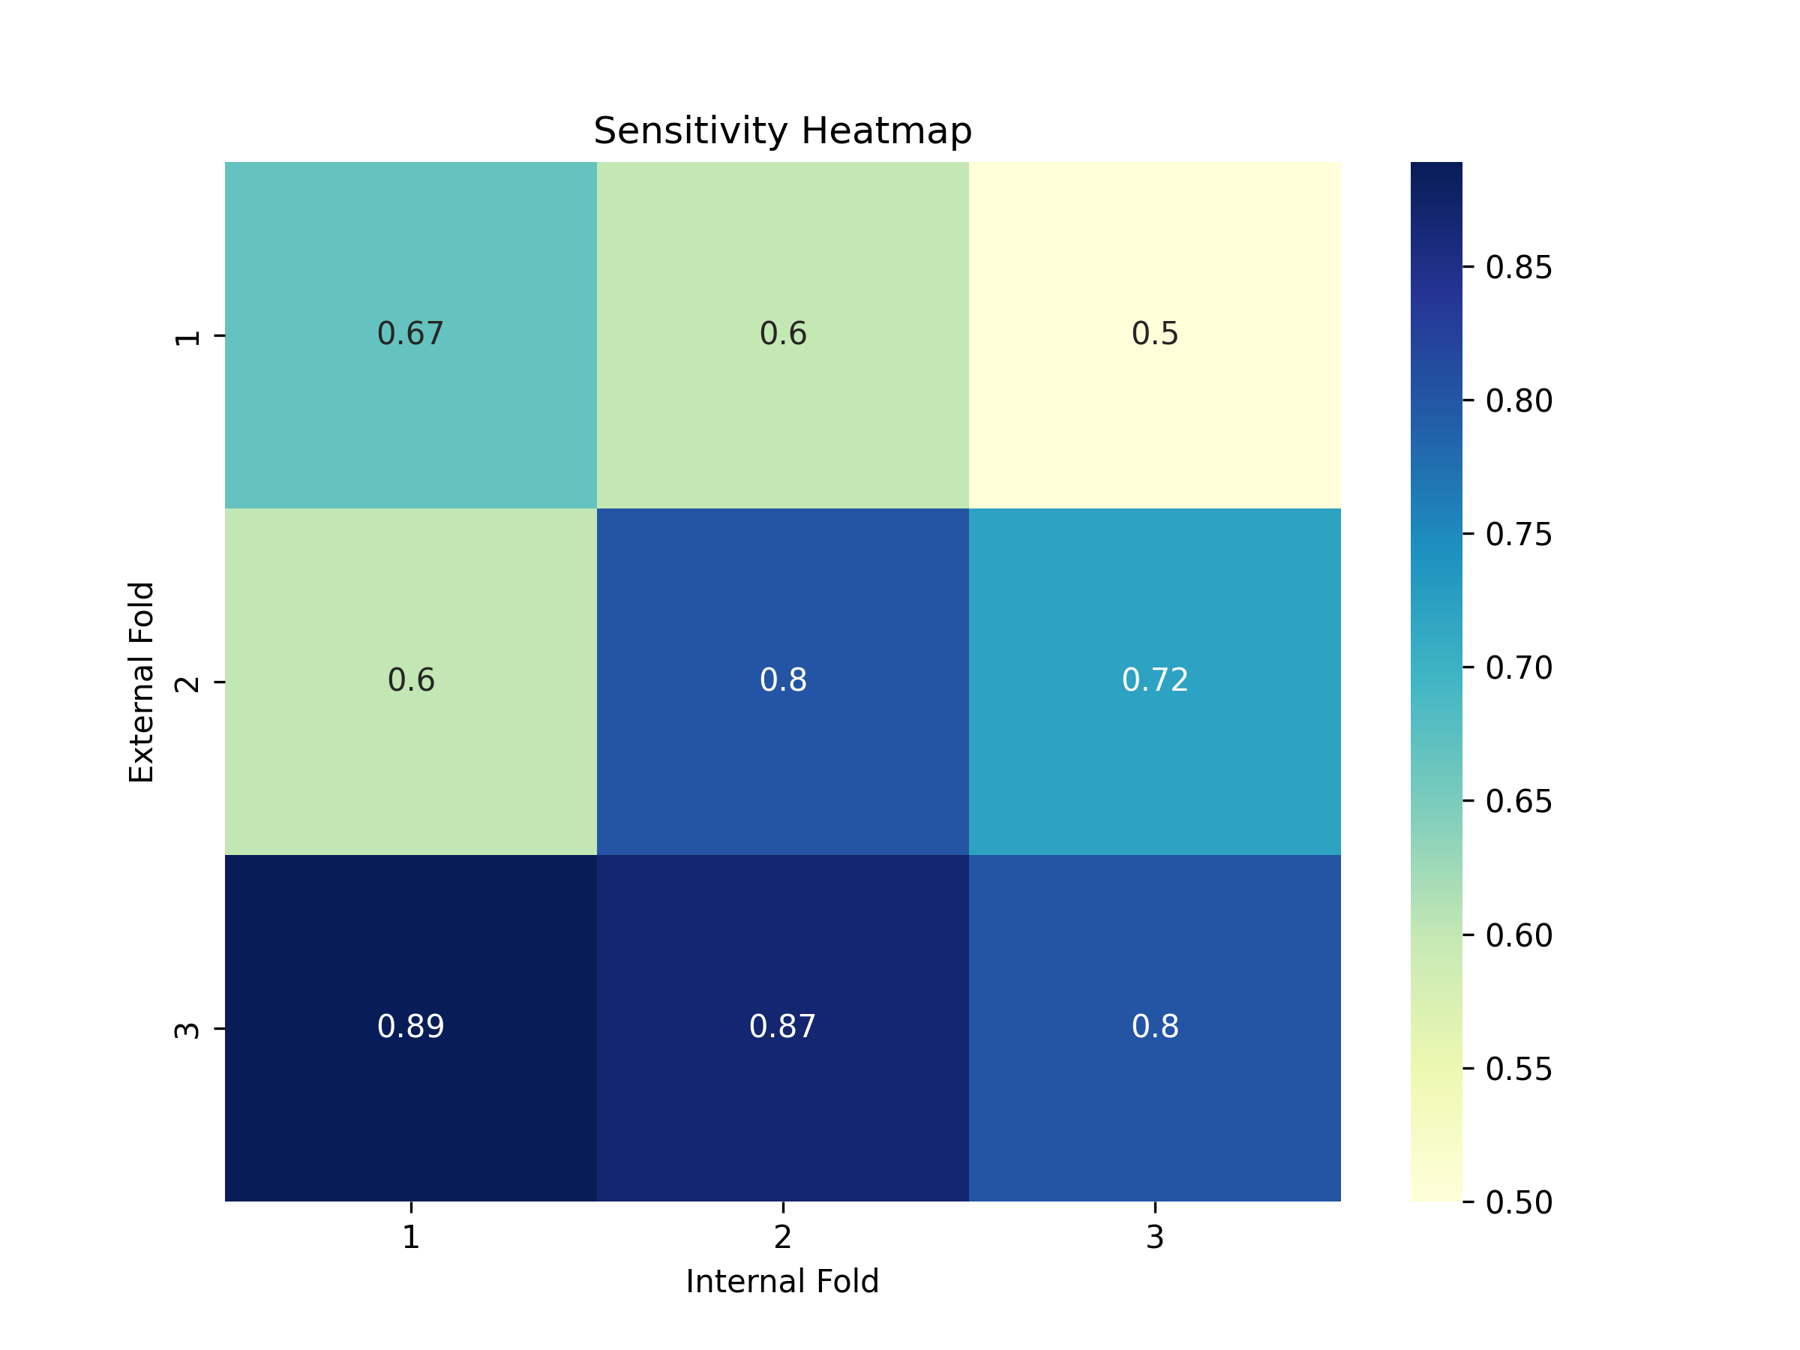
\includegraphics[width=1\linewidth]{figs/Picture4.png}
%     \caption{The testing sensitivity heatmap of CNN-based model (top) and hybrid ViT-CNN model (bottom), training setting keeps same (batch size = 8, learning rate = 0.0001, epoch = 5) }
%     \label{fig:enter-label}
% \end{figure}

%\begin{figure*}[htbp]
%    \centering
%    \begin{subfigure}[b]{0.4\textwidth}
%        \centering
%        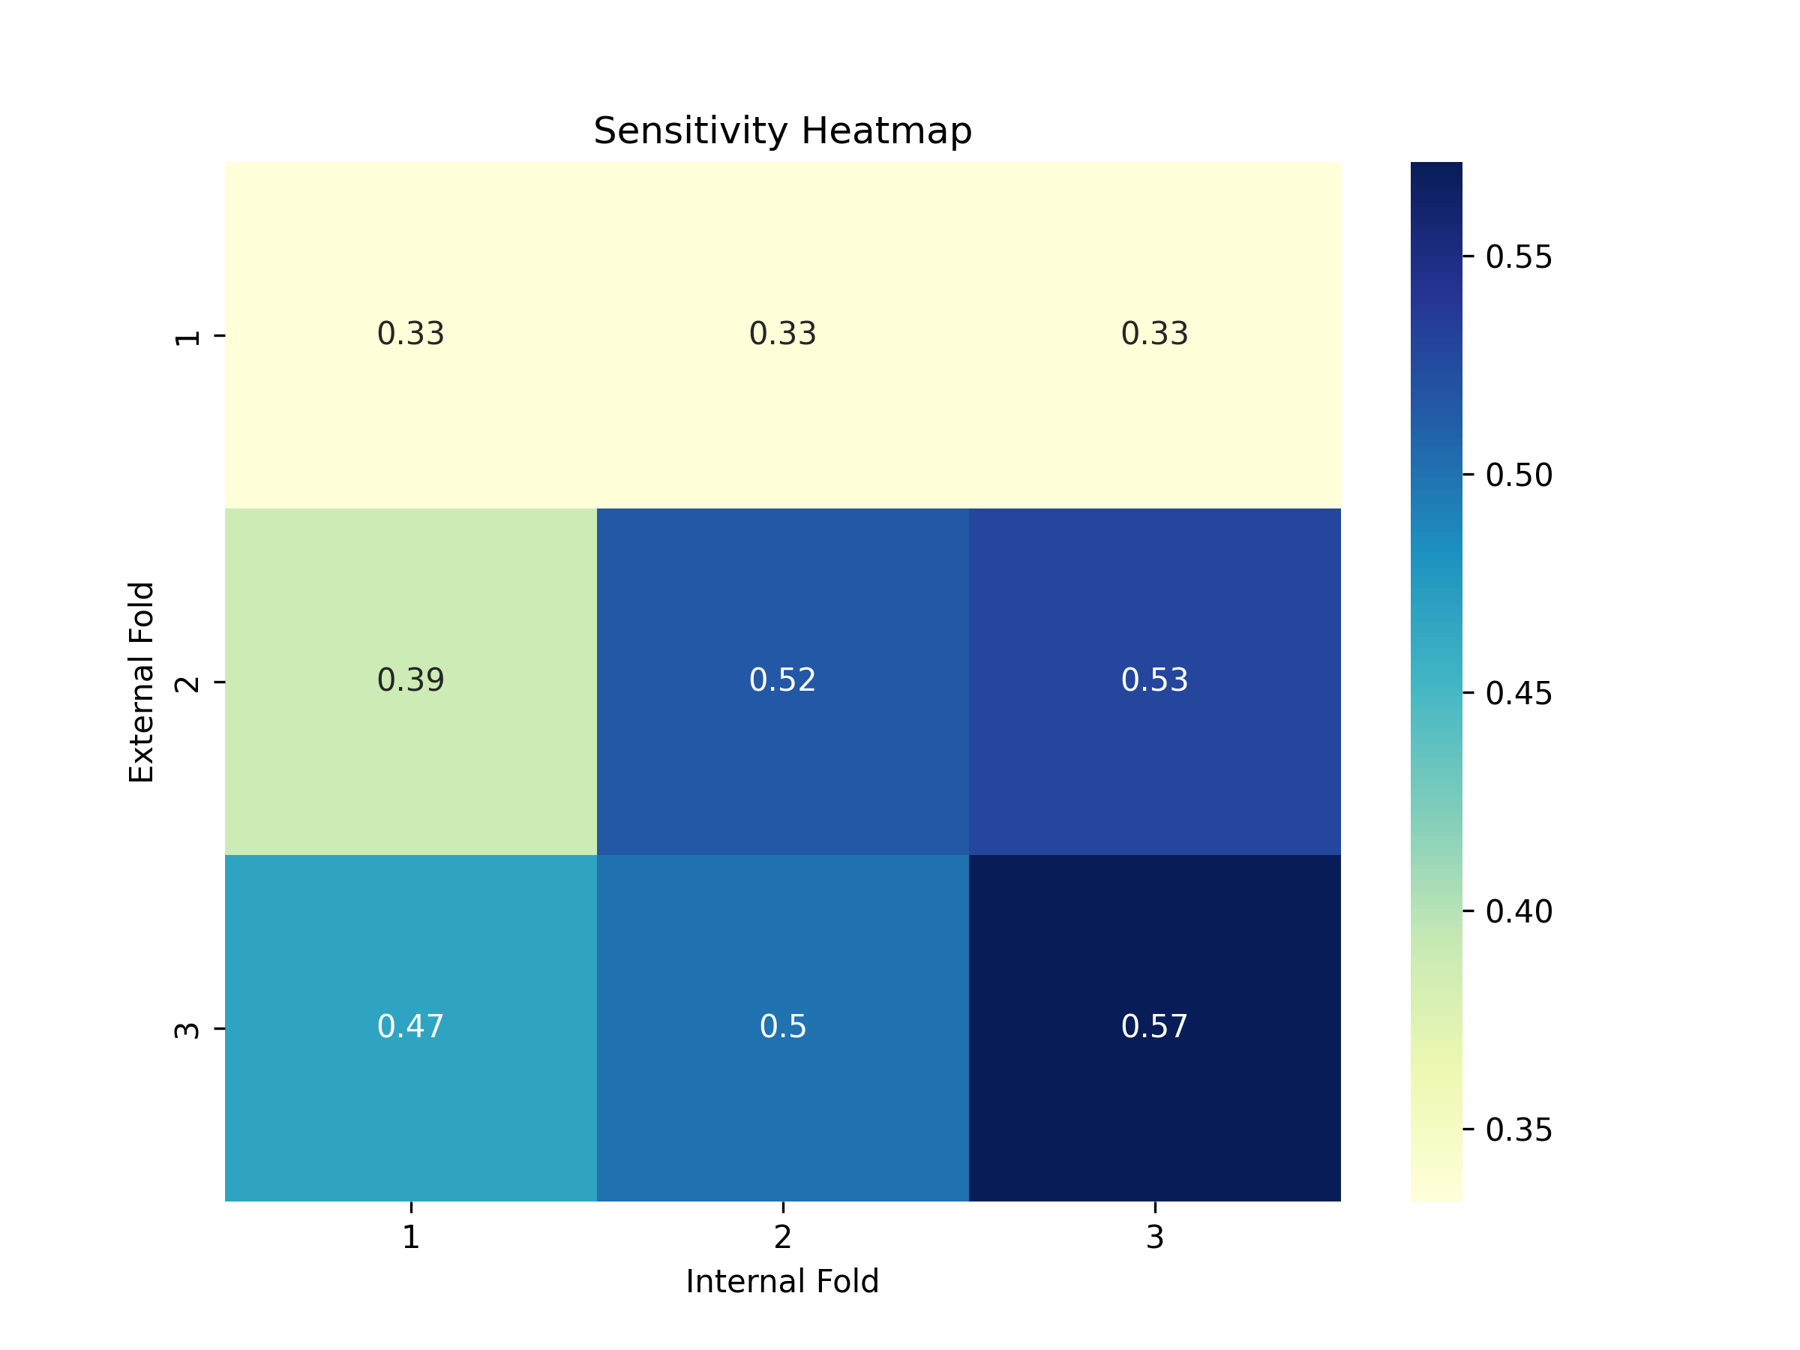
\includegraphics[width=\linewidth]{figs/Picture3.png}
%        \caption{}
%        % \label{}
%    \end{subfigure}%
%    % \hfill
%    \begin{subfigure}[b]{0.4\textwidth}
%        \centering
%        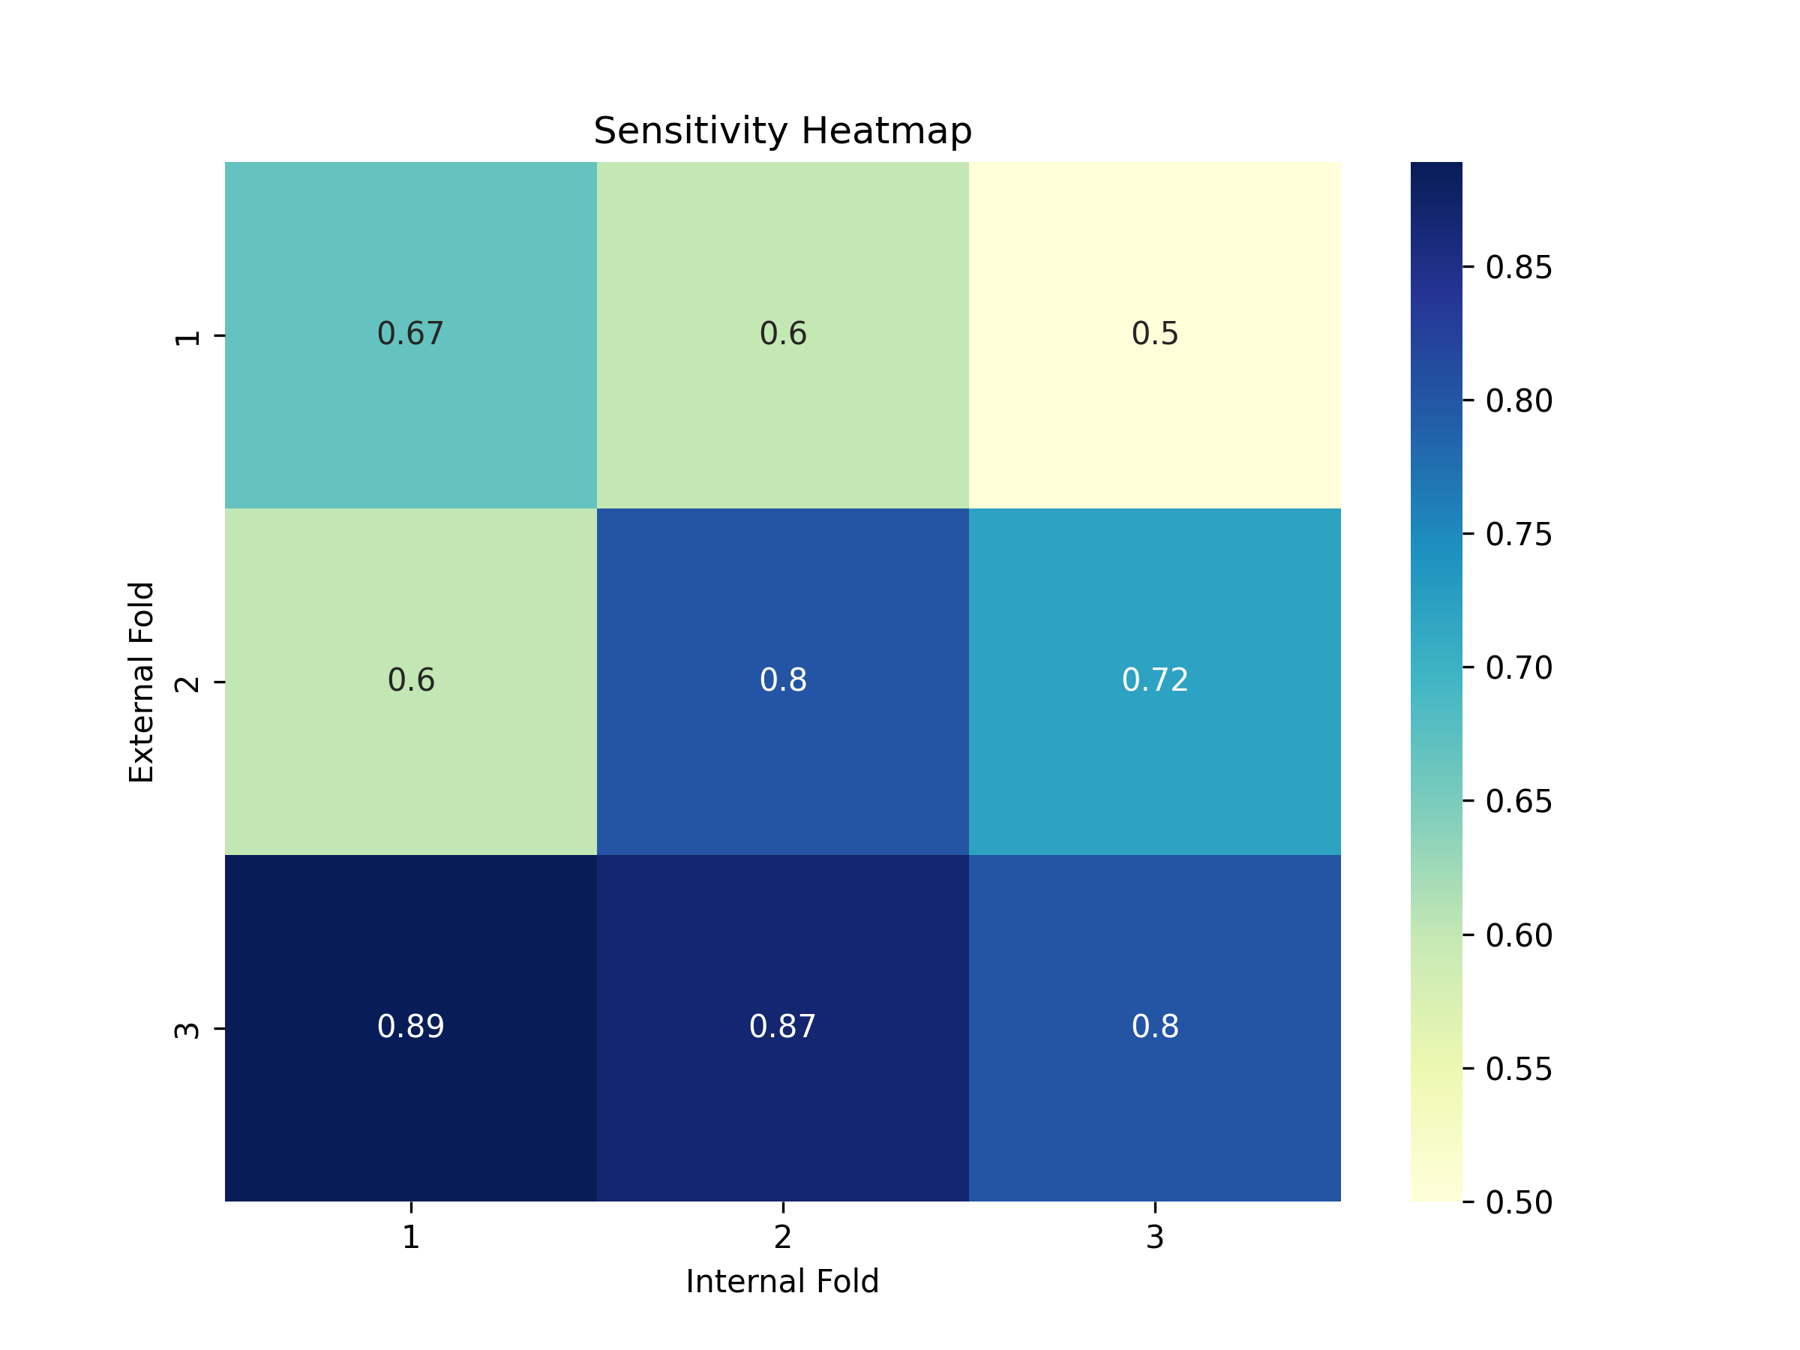
\includegraphics[width=\linewidth]{figs/Picture4.png}
%        \caption{}
%        % \label{}
%    \end{subfigure}
%    \caption{The testing sensitivity heatmap of CNN-based model (top) and hybrid ViT-CNN model (bottom), %training setting keeps same (batch size = 8, learning rate = 0.0001, epoch = 5)}
%    \label{fig:enter-label}
%\end{figure*}


\subsection{AD Progression}
The hyperparameter optimization for PCA and SVM had the best sensitivity scores for the 7 timepoints for 50 components for SVM. The PCA number of components (2, 10 or 25) had similar scores. 

%\begin{figure*}
%    \centering
%    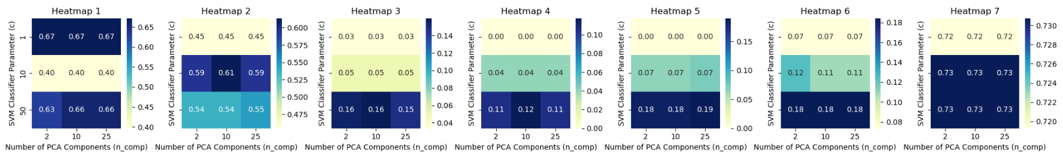
\includegraphics[width=1\linewidth]{figs/Picture7.png} 
    
%\end{figure*}
%\begin{figure*}
%    \centering
%    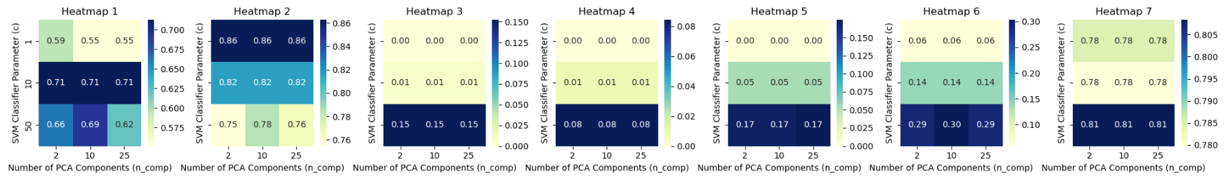
\includegraphics[width=1\linewidth]{figs/Picture8.png}
%    \caption{The AD Progression hyperparameter optimization for PCA and SVM components. The top row is the result for the CNN model and the bottom row for ViT model’s feature extraction. }
%    \label{fig:enter-label}
%\end{figure*}

Furthermore, comparing the training versus testing sensitivity scores for the three models (CNN, ViT, ResNet18-ViT) feature extractions fluctuated across timepoints. Timepoint 1, 2 and 7 the ViT model had higher test sensitivity. Timepoint 3, 4, 5 and 6 both models performed poorly with test sensitivity $ \leq 50 \%$. Next, we removed the PCA dimensionality reduction and just used SVM with 50 components. Here not only timepoint 2 and 7 but also 1 had higher test sensitivity for ViT model. The performance for timepoints 3, 4, 5 and 6 for both models improved for both models, where timepoint 6 CNN performed better than ViT model.  The hybrd ResNet18-ViT performed worse than CNN and ViT with test sensitivity $\leq 22 \% $ and training sensitivity \textgreater $50 \% $ for timepoint 4,5, and 7 ($57, 77, 63 \%$).  

%\begin{figure*}
%    \centering
%    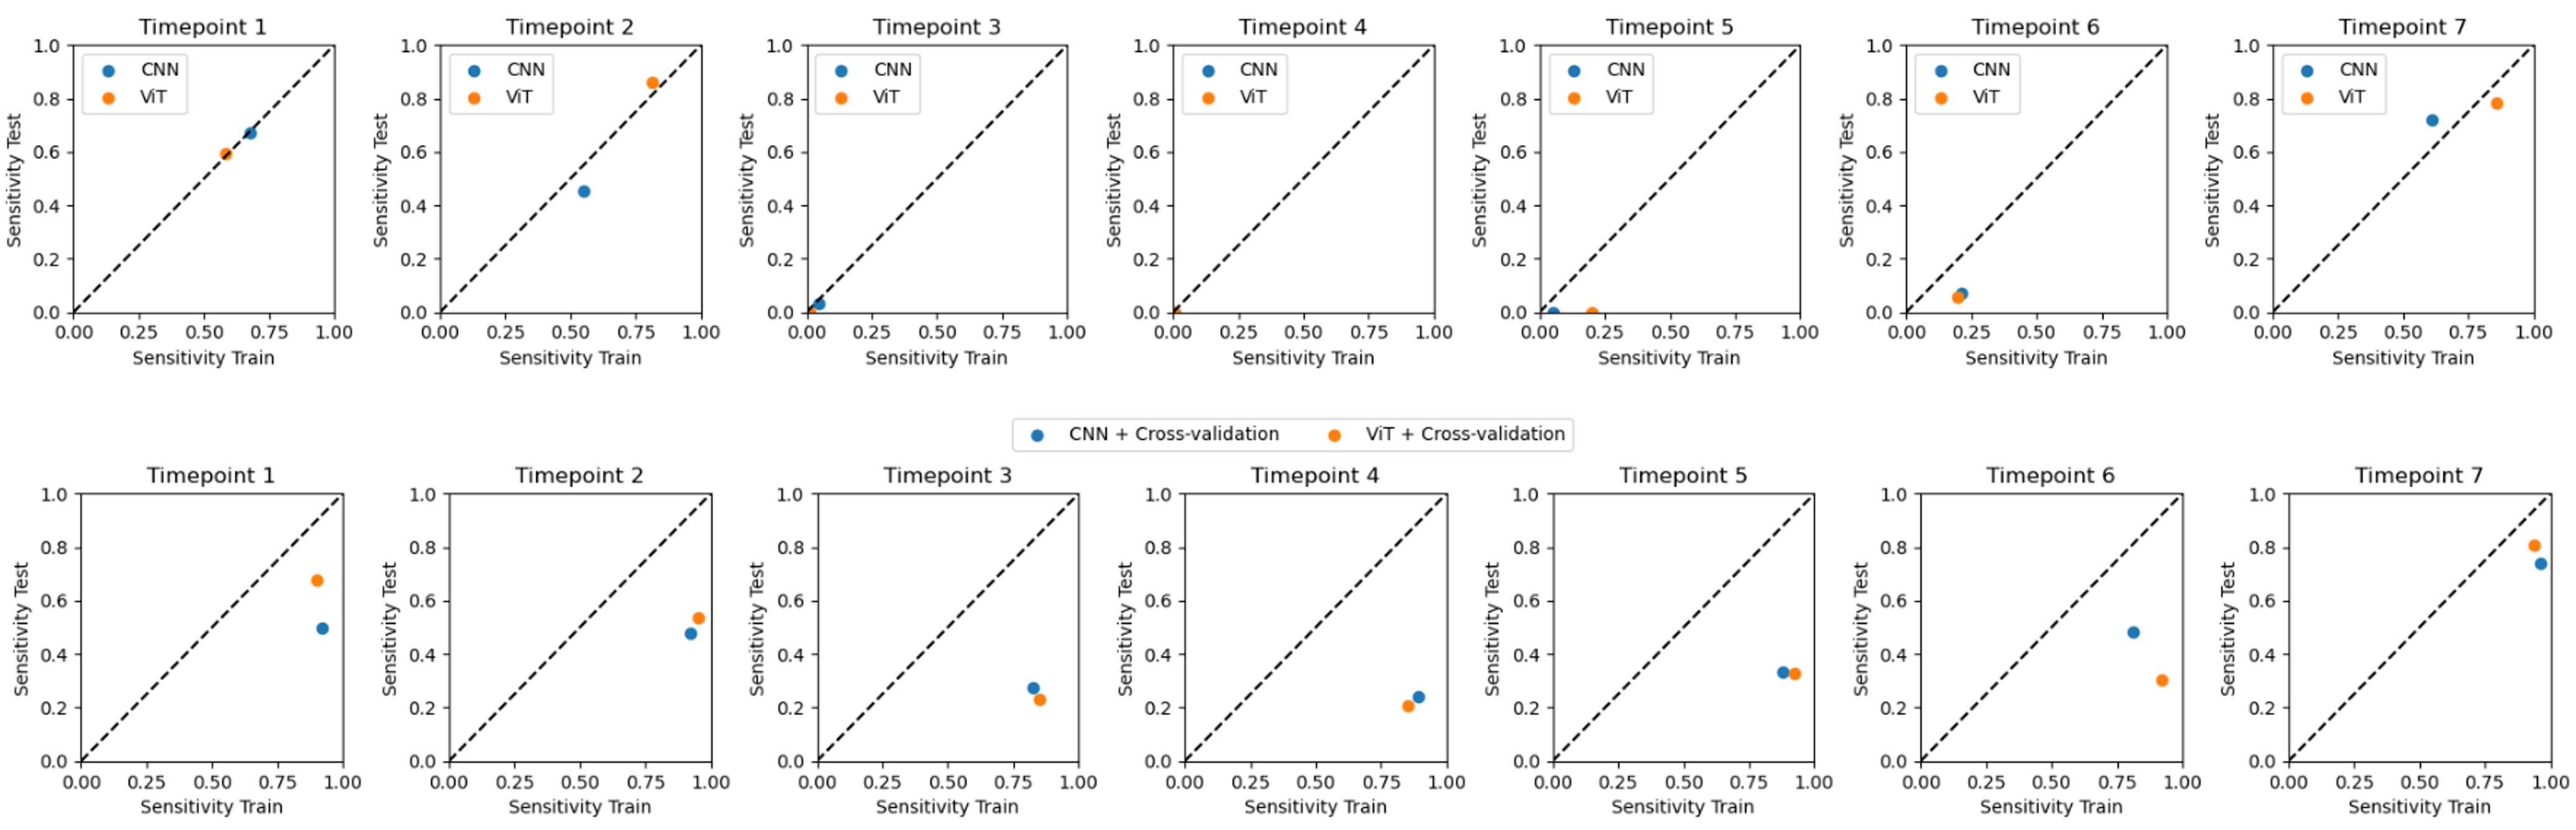
\includegraphics[width=1\linewidth]{figs/Picture15.png}
%    \caption{The AD Progression Predictivity Plots for feature extraction with CNN vs. ViT. The top row shows the training vs. testing sensitivity scores for the 7 timepoints. The bottom row is without PCA and SVM with 50 components.  }
%    \label{fig:enter-label}
%\end{figure*}

\subsection{Each Modality’s Contribution}
\textbf{AD Classification}
To investigate the impact of different modalities on the performance of AD classification, we conduct experiments using single modalities and their combinations in the proposed hybrid ViT-CNN model and keep the same experimental setting for each experiment. The testing results provide valuable insights into the role of each modality in AD diagnosis. 

As shown in Table 1, the testing results revealed distinct performance metrics for each modality and their combinations, When MRI and PET features are combined in the CNN and ViT components, they substantially enhance classification performance. For example, the PET outperforms MRI with an accuracy of 59\% compared to MRI’s 54\%. PET also exhibits higher F1 scores and sensitivity. Furthermore, when combining all the modalities the accuracy for the combined MRI and PET model is 63\%, which is superior to the results of the single modalities. The combined approach also shows improvements in F1 scores and sensitivity. 


\begin{table}[ht]
% \centering
\caption{Modality testing results comparison using the hybrid ViT-CNN model in the same experiments settings with same subjects of two different datasets.}\label{tab:results-cls-modality}
\resizebox{0.48\textwidth}{!}{%
\begin{tabular}{lcccc}
\toprule
\textbf{Modality} & \textbf{Dataset} & \textbf{Accuracy} & \textbf{F1 Score} & \textbf{Sensitivity} \\
\midrule
MRI & MaskMRI+PET & 0.5479 & 0.4489 & 0.6139 \\
PET & MaskMRI+PET & 0.5902 & 0.5526 & 0.7466 \\
MRI \& PET & MaskMRI+PET & 0.6330 & 0.5818 & 0.8103 \\
MRI \& PET \& EHR & MaskMRI+PET & 0.6393 & 0.5881 & 0.8052 \\
MRI \& PET \& EHR \& Gen. & MaskMRI+PET & 0.6393 & 0.5881 & 0.8052 \\
\midrule
MRI & MRI+PET & 0.5725 & 0.4169 & 0.6537 \\
PET & MRI+PET & 0.5802 & 0.4813 & 0.6922 \\
MRI \& PET & MRI+PET & \textbf{0.6031} & \textbf{0.5774} & \textbf{0.7646} \\
MRI \& PET \& EHR & MRI+PET & \textbf{0.6031} & \textbf{0.5774} & \textbf{0.7646} \\
MRI \& PET \& EHR \& Gen. & MRI+PET & \textbf{0.6031} & \textbf{0.5774} & \textbf{0.7646} \\
\bottomrule
\end{tabular}
}
\end{table}

For the feature contribution results, after ranking the highest 20 features from all of them, we can get the PET features (pet-cnn-1310594, pet-cnn-326784, and pet-cnn-1034881) in the CNN component demonstrated the top three importance shown in the right plot from Figure 3. Notably, there is a PET feature from pretrained ViT model also has a high feature importance. CNN’s PET features account for the largest proportion among these 20 features. From overall, by selecting the top 768 features from MRI-CNN and PET-CNN which match the quantity of the MRI and PET in ViT model. We can observe that the contribution of the first 768 features of PET-CNN is nearly 50\% higher than that of the first 768 features of MRI-CNN. In addition, the PET-ViT feature also plays a certain role, followed by the MRI-ViT feature. However, EHR features showed the least contribution, which could be attributed to the limited feature types. 

  \begin{figure*}
     \centering
     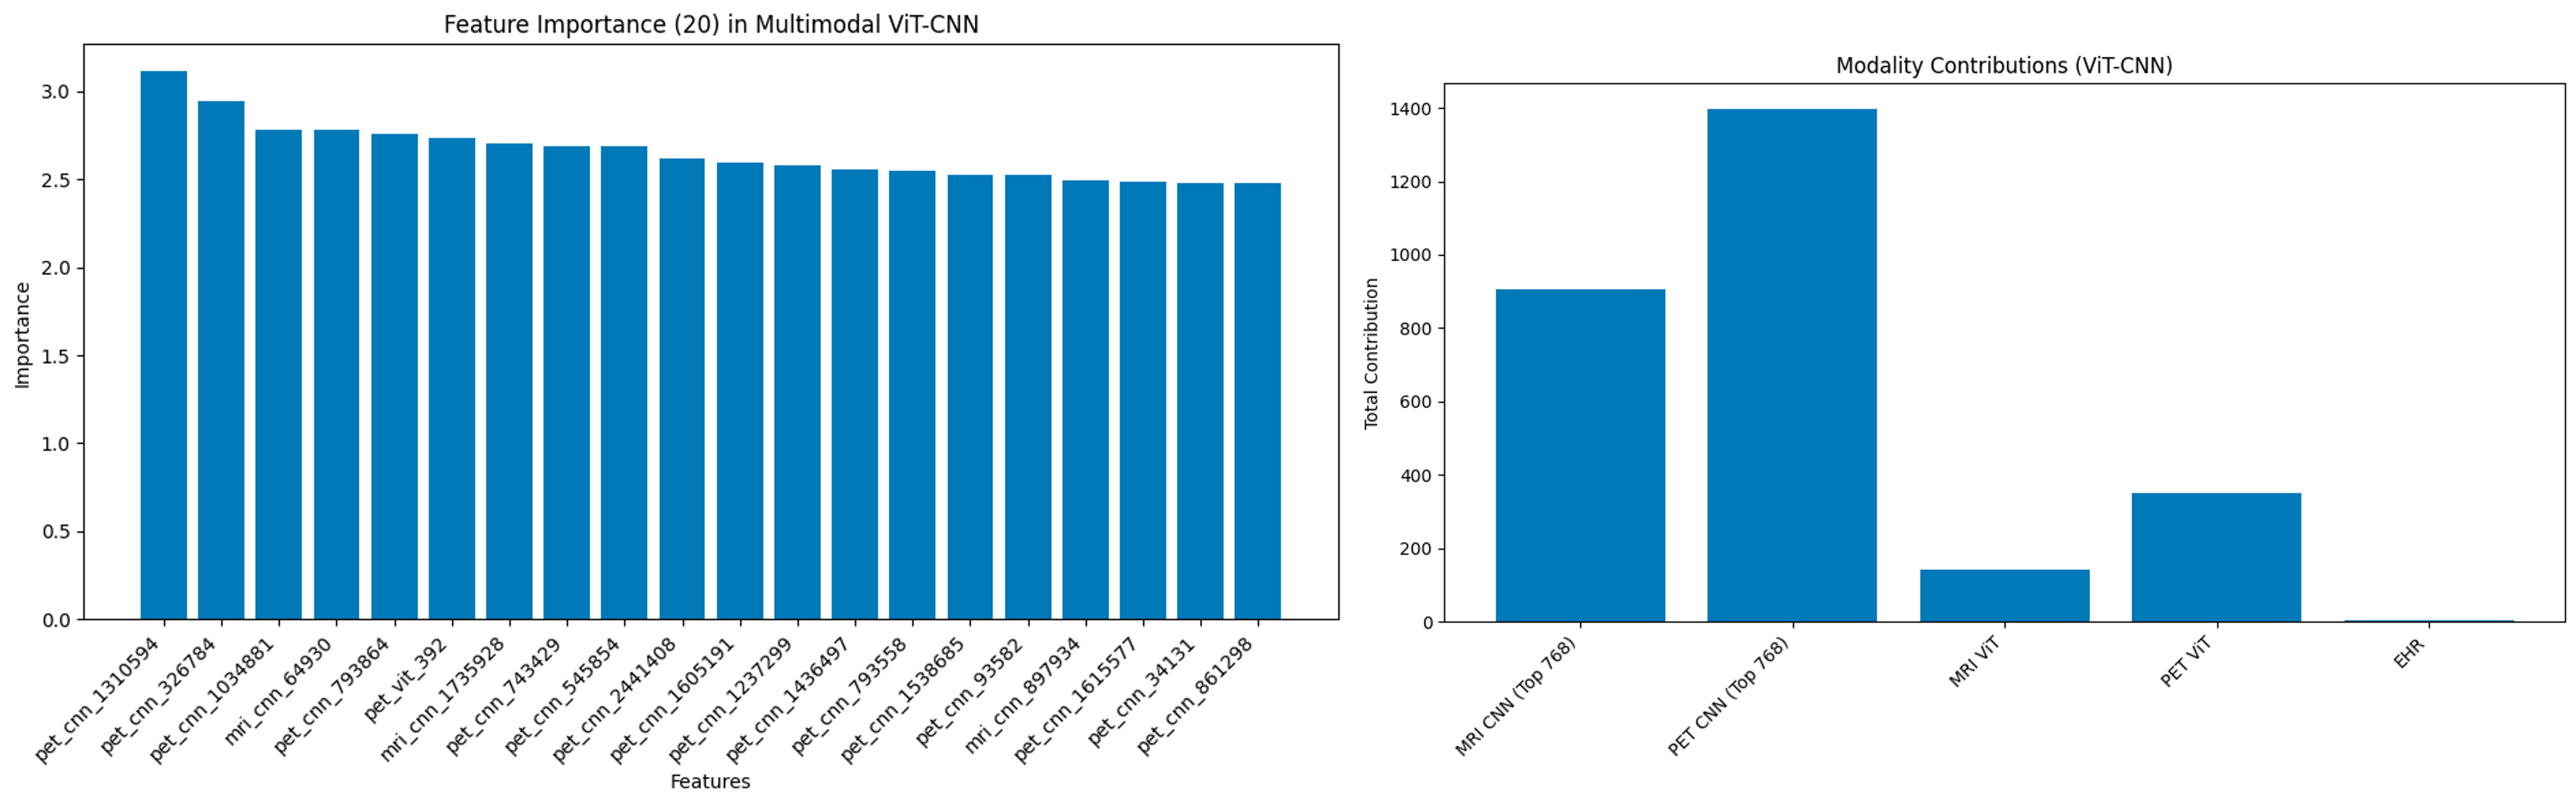
\includegraphics[width=1\linewidth]{figs/Picture16.png}
     \caption{Modality contribution analysis by ranking all the feature importances from CNN and ViT of MRI and PET images. }
    \label{fig:enter-label}
 \end{figure*}
 
\textbf{AD Progression}
To test the contribution of each modality and their combination we tested the classification based on features extracted from CNN vs. ViT from MRI, PET, MRI \& PET, HER \& Genetic, and MRI \& PET \& EHR \& Genetic. There are oscillations across the 7 timepoints for the three metrics of accuracy, F1 and Test Sensitivity (Table 2 and Figure 4).  

The MRI accuracy for CNN is between 50 to 55\%, while for ViT it is between 45 to 60\%. The PET accuracy for CNN is between 42 to 55\%, while 45 to 58\% for ViT. The combination of MRI and PET for CNN is 45 to 58\%, while for ViT is 44 to 59\%. The EHR and Genetic accuracy for CNN is 37 to 63\%, while for ViT 37 to 63\%. The combination of all modalities for CNN is 48 to 62\%, while for ViT is 43 to 59\%.  

The F1 scores for MRI data with CNN range from 20\% to 59\%, while with ViT, they range from 26\% to 70\%. For PET data, the F1 scores with CNN range from 32\% to 68\%, whereas with ViT, they range from 21\% to 65\%. Combining MRI and PET data, the F1 scores with CNN range from 23\% to 65\%, whereas with ViT, they range from 22\% to 60\%. For EHR and Genetic data, the F1 scores with CNN range from 0\% to 59\%, like ViT. Finally, combining all modalities, the F1 scores with CNN range from 52\% to 65\%, whereas with ViT, they range from 23\% to 60\%. 

\begin{table*}[ht]
% \centering
\caption{The performance of modalities and their combination for CNN and ViT models for timepoints 1 to 7 (t1-7). The top table is the CNN accuracy, F1 score and Test sensitivity. The bottom table is the ViT accuracy, F1 score and Test sensitivity.}\label{tab:results-cls-modality}
\resizebox{\textwidth}{!}{%
\begin{tabular}{lccc}
\toprule
\textbf{Modality: CNN}& \textbf{Accuracy t1-7}& \textbf{F1 Score t1-7}& \textbf{Sensitivity t1-7}\\
\midrule
MRI & 54,55,50,55,50,50,50& 51,57,26,20,36,32,59& 57,58,35,20,31,34,79\\
PET & 42,55,52,58,44,48,52& 32,58,37,33,36,45,68& 33,60,38,33,36,45,68\\
MRI \& PET & 45,45,50,53,45,48,58& 45,44,29,23,39,42,65& 52,45,27,21,35,51,76\\
EHR \&  Genetic& 49,51,59,63,37,39,40& 43,59,0,0,0,0,47& 53,68,0,0,0,0,72\\
MRI \& PET \& EHR \& Genetic& 52,62,54,54,48,48,54& 60,65,59,60,58,52,57& 74,64,71,71,74,63,64\\
\midrule
 \textbf{Modality: ViT}& \textbf{Accuracy t1-7}& \textbf{F1 Score t1-7}&\textbf{Sensitivity t1-7}\\
\midrule
MRI & 51,52,52,51,47,45,60& 47,58,30,26,31,31,70& 52,62,28,25,26,30,93\\
PET & 50,48,45,50,54,50,58& 45,49,21,25,44,38,65& 56,50,20,22,41,42,85\\
MRI \& PET & 59,47,48,48,50,44,50& 58,53,25,22,37,34,60& 68,58,23,19,34,33,80\\
EHR \&  Genetic
& 49,51,59,63,37,39,40& 43,59,0,0,0,0,47& 53,68,0,0,0,0,72\\
MRI \& PET \& EHR \& Genetic& 59,57,48,49,48,43,50& 58,58,26,23,36,33,60& 68,54,23,21,33,30,81\\
\toprule
 \textbf{Modality: ResNet18-ViT}& \textbf{Accuracy t1-7}& \textbf{F1 Score t1-7}&\textbf{Sensitivity t1-7}\\
\midrule
 MRI 
& 50, 50, 53, 60, 47, 47, 62
& 50, 53, 34, 34, 37, 33, 68
&62, 56, 36, 34, 37, 30, 80
\\
 PET 
& 56, 48, 45, 50, 53, 43, 42
& 42, 45, 31, 24, 29, 31, 56
&40, 43, 31, 25, 25, 34, 79
\\
 MRI \& PET 
& 55, 46, 42, 53, 48, 41, 56& 43, 48, 25, 27, 33, 30, 66&51, 49, 26, 26, 29, 31, 87\\
 EHR \&  Genetic
& 49, 51, 59, 63, 37, 39, 40
& 43, 59, 0, 0, 3, 3, 47
&53, 69, 0, 0, 2, 3, 72
\\
 MRI \& PET \& EHR \& Genetic& 60, 44, 48, 48, 47, 45, 48& 52, 42, 25, 31, 32, 36, 58&62, 45, 23, 29, 28, 40, 73\\
\bottomrule
\end{tabular}
}
\end{table*}.\label{tab:results-cls-modality}

Similarly, the Test Sensitivity scores for MRI data with CNN range from 20\% to 79\%, while with ViT, they range from 25\% to 93\%. For PET data, the Test Sensitivity scores with CNN range from 33\% to 68\%, whereas with ViT, they range from 20\% to 85\%. Combining MRI and PET data, the Test Sensitivity scores with CNN range from 21\% to 76\%, whereas with ViT, they range from 19\% to 80\%. For EHR and Genetic data, the Test Sensitivity scores with CNN range from 0\% to 72\%, like ViT. Finally, combining all modalities, the Test Sensitivity scores with CNN range from 63\% to 74\%, whereas with ViT, they range from 21\% to 81\%. 

\begin{figure*}
    \centering
    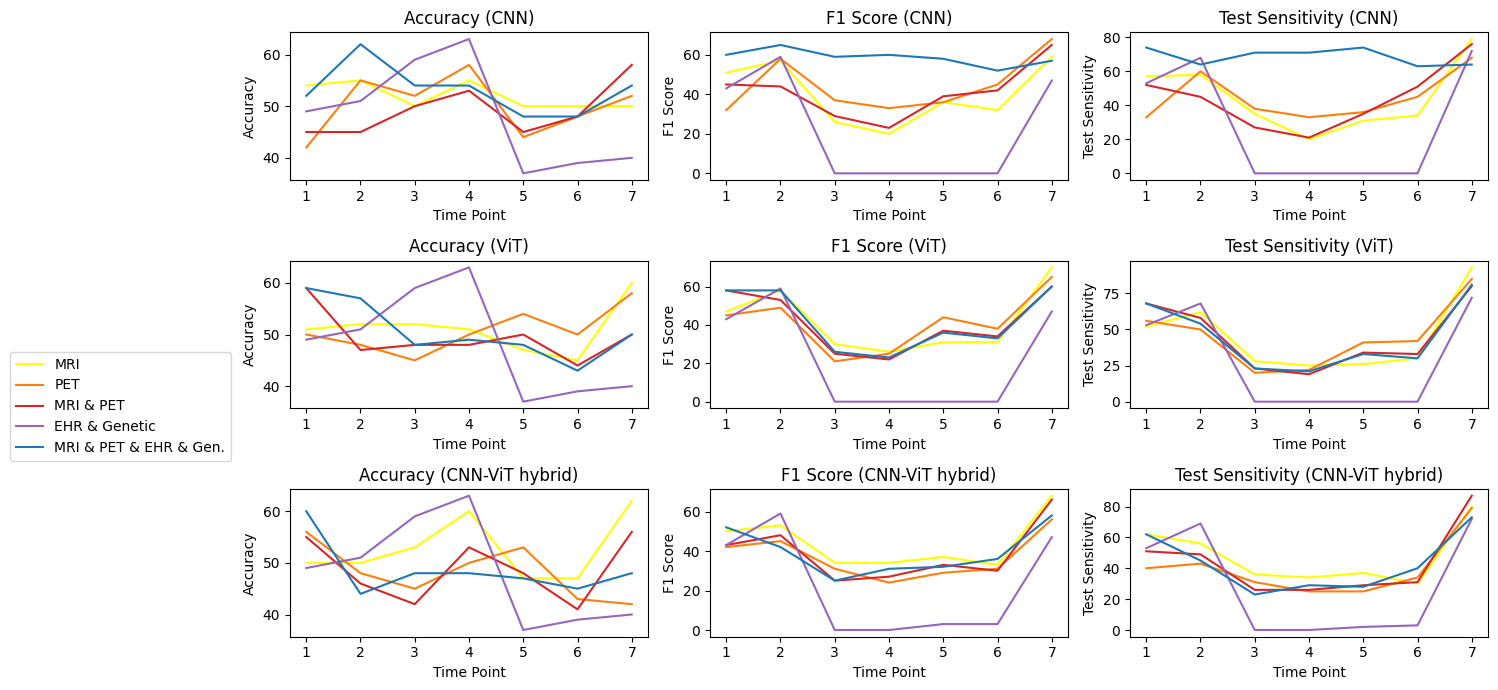
\includegraphics[width=1\linewidth]{figs/Picture17_1.png}
    \caption{The plot of accuracy, F1 score and Test Sensitivity for CNN and ViT feature extractions for each modality and their combinations }
    \label{fig:enter-label}
\end{figure*}
%\vspace{-2mm}

\section{Discussion}
\label{sec:discussion}
\subsection{AD Classification}
A key innovation of our approach is to exploit complementary information from CNN and ViT. CNN is good at capturing local features, while ViT is good at modeling global dependencies. By combining these two types of features, our model can represent brain imaging data more comprehensively, thereby improving the performance of AD classification. Furthermore, by leveraging pre-trained ViT models, our approach can effectively leverage universal visual representations learned on large-scale datasets. 

We found that the hybrid ViT-CNN model showed better consistency, and its validation results were closer to the test results (validation accuracy 77\%, test accuracy 70\%). In contrast, the performance of the CNN encoder model on the validation set and test set differs greatly. This shows that the hybrid ViT-CNN model has stable generalization ability. 

It is worth noting that the ViT model alone has the lowest performance. We believe this may be because the pre-trained ViT model is trained on a large-scale natural image dataset, and medical imaging data is significantly different from natural images. 

By incorporating a pretrained ViT alongside the CNN encoder, the hybrid model achieves a remarkable increase in sensitivity from approximately 52\% to around 80\%, while maintaining consistent hyperparameters. This superior performance can be attributed to the pretrained ViT's ability to facilitate effective multi-modality integration and the concatenation of diverse features extracted from both the CNN and ViT. The promising results suggest that the hybrid ViT-CNN model has the potential to become a state-of-the-art approach for AD classification. Visualization techniques such as t-SNE and Grad-Cam will further elucidate the important regions learned by the model, contributing to the development of more accurate and reliable AD diagnosis techniques. 

\subsection{AD Progression}
The hyperparameter optimization results suggest that dimensionality reduction using PCA does not help the classification performance. The SVM with 50 components outperforms 1 and 10 components. In addition, although for 3 out of 7 timepoints ViT had higher Test Sensitivity scores than CNN, for timepoints 3-5 they were similar and for timepoint 6 CNN had higher Test Sensitivity scores. Overall, the test sensitivity scores were lower than expected. This could be since these models were pretrained on non-medical images. It is essential to do transfer learning and train them on medical images before doing feature extraction. 

The hybrid model, ResNet18-ViT, did go through transfer learning. One model got trained on MRI images from all time points for MRI feature extraction and a separate model got transfer learning training on PET images from all time points for PET feature extraction. Even though, theoretically the hybrid model should outperform the CNN and ViT models, but the test sensitivity scores were below 22 \% for the seven timepoints and training sensitivity got obove 50 \% for three out of seven timepoints. Therefore, for this dataset the ViT model outperformed the CNN and the hybrid model performed worse on the sensitivity scores. 

\subsection{Modality Contributions} 

\textbf{AD Classification: }

In the single modality setting, PET demonstrated superior performance compared to MRI. The accuracy of PET reached 59\%, surpassing that of MRI at 55\%. Moreover, PET exhibited higher F1 score and sensitivity, further highlighting its diagnostic value in AD classification. These findings underscore the importance of PET imaging in capturing AD-related pathological changes. However, in spirit of transparency the MRI images in the dataset we used were masks and not true MRI images. We are re-running our analysis with a hybrid dataset that combines good MRI images with PET images and will report our updated results in future.  

Moving on to multimodal modeling, the combination of MRI and PET improved significantly. The accuracy of the MRI and PET combined model reached 63\%, outperforming the individual modalities. The F1 score and sensitivity also witnessed similar enhancements. This suggests that the complementary information provided by MRI and PET contributes to a more comprehensive representation of AD characteristics, leading to improved classification performance. 

Furthermore, by comparing the results across different hyperparameter settings, we observed that multimodal models exhibited greater stability. Even with the inclusion of EHR and genomic data, the performance remained comparable to the MRI and PET combination, indicating the robustness of multimodal models to data variations and noise. 

Regarding the limited improvement brought by the addition of EHR and genomic data, the analysis points to the limitation on the number of feature types  as a potential factor. Acquiring large-scale EHR and genomic data poses greater challenges compared to imaging data. Therefore, future work should focus on collecting more comprehensive EHR and genomic samples to fully harness their potential in AD classification. 

In conclusion, the modality analysis conducted through testing results corroborates our previous observations. PET excels in single modality performance, while multimodal modeling significantly enhances the accuracy and stability of AD classification. Although the contribution of EHR and genomic data is limited in the current study, it highlights the importance of gathering more extensive and high-quality multimodal data. By integrating imaging, clinical, and genomic information, we can strive towards building more precise and robust models for AD diagnosis. 

As shown in Figure 6, we also investigated the contribution of different modalities to Alzheimer's Disease (AD) classification, we conducted feature permutation experiments in the multimodal ViT-CNN model. Our analysis showed that features of PET in the CNN component had the highest importance, corroborating earlier findings that PET is effective in AD diagnosis. MRI and PET features within the CNN and ViT components also made substantial contributions, particularly when combined, highlighting the model's ability to utilize complementary information from both modalities to enhance classification performance. 

In contrast, EHR features contributed the least, likely due to the limited sample size in our dataset, which may not fully represent the potential of EHR in AD diagnosis. This emphasizes the need for larger EHR datasets to better explore its utility. 

The bar graph illustrating modality contributions clearly shows PET as the most significant contributor, followed by combined PET \& MRI features. The findings validate our hypothesis that multimodal approaches improve classification performance and stability. 

Future research should aim to expand EHR data collection and explore methods to better integrate it with imaging modalities to enhance the performance of multimodal models. Overall, these insights confirm the importance of multimodal modeling in AD diagnosis and underscore the need for comprehensive datasets that include imaging, clinical, and genomic information. 

\textbf{AD Progression: }

The contribution of modalities and their performance metrics of accuracy, F1 score, and Test Sensitivity oscillated across timepoints and the range of values for CNN, ViT and ResNet18-ViT were similar. One strange observation is that the F1 score and Test Sensitivity for EHR and Genetic features were zero for timepoint 3 to 6 regardless of the model used (\autoref{fig:ADprogression}). The EHR consisted of binary biological sex and normalized age variable and the genetic feature is the normalized polygentic hazard score (PHS). Since the sex and and PHS does not change across time points, these features would not theoretically be useful in predicting conversion from sMCI to pMCI. However, age should be a predictive feature. The age variable has a mean of 77.2, min of 55, 25\% of 73, median of 77, 75\% of 82 and max of 96. One possibility could be that timepoints 3-6 lies in the 73-82 years of age and most patients are already pMCI and there is not a lot of switches between sMCI to pMCI. 

\
%\vspace{-2mm}

\section{Conclusion: Advancements in Multimodal Brain Data Analysis for Alzheimer’s Disease Prediction.}
Our study presents a novel approach to Alzheimer’s Disease (AD) classification by harnessing the complementary strengths of Convolutional Neural Networks (CNN) and Vision Transformers (ViT). The hybrid ViT-CNN model capitalizes on CNN's capability to capture local features and ViT's strength in modeling global dependencies, resulting in improved performance and stability in AD classification tasks. The hybrid model exhibits superior consistency and generalization compared to individual models, and the incorporation of a pre-trained ViT significantly enhances sensitivity, underscoring its effectiveness in multimodal data integration.

While PET proved to be the most effective single modality, the combination of MRI and PET in a multimodal framework yielded even greater improvements in classification accuracy and robustness. However, the contribution of Electronic Health Records (EHR) and genomic data was limited, indicating the need for larger and more diverse datasets to fully realize the potential of these modalities in AD diagnosis.

Overall, our findings highlight the critical role of multimodal approaches in advancing AD classification and suggest promising directions for future research. These include optimizing the integration of diverse data modalities, improving dataset quality and size, and refining transfer learning techniques to develop more precise, stable, and interpretable models for early AD diagnosis and progression prediction.
%\vspace{-2mm}

\section{References}
\bibliographystyle{ieeetr}
\bibliography{Bibliography}

\end{document}


